
Название:
Учёт групп органов управления при синтезе тензорных сигналов управляющих воздействий в задачах управления движением.

Аннотация:


1. Введение.

Системы управления, работающие с сигналами, выраженными в векторном виде требуют синтеза векторных управляющих воздействий. Такие сигналы могут меняться как по модулю, так и по направлению. На практике обычно используются органы управления со скалярными, выраженными единственным параметром сигналами. Построение же векторного управляющего воздействия достигается применением нескольких совместно действующих скалярных сигналов. По сути, способность групп органов управления генерировать разнонаправленные сигналы, при том, что каждый из органов управления по отдельности способен к генерации сигнала только по одному конкретному направлению является эмерджентным свойством и потому требует комплексного рассмотрения всей группы как единого объекта.

2. Обзор.

Группы органов управления для совместной генерации управляющего воздействия широко применяется в технических решениях. В качестве примеров можно рассмотреть ракеты, имеющие несколько параллельных реактивных двигателей, мультикоптеры, строящие управления за счёт комбинации смещенных относительно центра масс двигателей, способных решить задачу только в составе группы. К числу этих объектов также относятся роботы манипуляторы, для которых перемещение хвата по заданной траектории требует совместной работы всех сочленений.

В данной статье рассмотрен вопрос учёта таких групп органов управления в контексте их применения в системах управления, основанных на векторно-тензорных сигналах. Вопрос применения тензорных сигналов рассматривался в предыдущей статье.

## Объекты управления.

Существуют две большие промышленно значимые группы объектов, в которых применяется подобное группирование управляющих сигналов.

Первая группа - свободно движущиеся летающие дроны, некоторые виды подводных роботов. Для этой группы управляющее воздействие строится в виде комбинации силовых воздействий двигателей, раскиданных по телу аппарата.

(Картинки)

Вторая группа - позиционеры, манипуляторы, управление выходными звеньями которых формируется из суперпозиции движений каждого сустава в отдельности.

(Картинки)

## Линейная группа органов управления.

Группой органов управления будем называть совокупность органов управления, совместно решающих задачу построения тензора управления $F = F(v_1, v_2, ..., v_n)$, где $n$ - количество органов управления. Если относительно управляющих воздействий органов управления выполняется принцип суперпозиции, то F является линейной комбинацией. Здесь и далее тензор $F$ выражается в векторном виде. 

\begin{equation}f_i=a^i_jv^j\end{equation}
\begin{equation} \label{lincomb}  F=AV\end{equation}

Вектором чувствительности будем называть приведенное к расчетному центру единичное воздействие, производимое органом управления.

Матрица $A$ является прямоугольным переменным матричным коэффициентом, образованным векторами чувствительностей органов управления. Количество её строк соответствует размерности вектора $F$, а количество столбцов числу органов управления в группе.

К системе линейных уравнений (\ref{lincomb}) сводится задача поиска управляющего воздействия отдельных органов группы, поскольку вектор желаемого управляющего воздействия $F$ является известным, а вектор воздействий органов группы $V$ требуется найти. Система может иметь одно решение, не иметь решений вовсе или же иметь множество решений. Случай отсутствия решений означает, что желаемое управление, требуемое от группы не может быть выполненно (вероятно, в силу физической несовместимости). Случай множества решений означает, что желаемое управление может быть достигнуто множеством способов. Поиск одного из множества решений возможен, например, с использованием метода поиска псевдообратной матрицы, однако вероятно, разработчик САУ захочет задать правила выбора конкретного решения из доступного множества.

Поиск оптимального решения на данном множестве требует введения функционала оптимизации и, возможно, дополнительных условий.

\begin{equation}\Phi(V) -> min\end{equation}
\begin{equation}AV = F\end{equation}
\begin{equation}CV <= d\end{equation}

Если $\Phi(V)$ - квадратичный функционал, а дополнительные условия отсутствуют, задача
 является задачей квадратичного программирования:

\begin{equation}\Phi(V) = \frac{1}{2}V^TQV+c^TV -> min\end{equation}
\begin{equation}AV = F\end{equation}

, которая разрешается в виде.
\begin{equation} \label{slau}
\begin{vmatrix}
Q & A^T\\
A & 0
\end{vmatrix}
\begin{bmatrix}
V\\
\lambda
\end{bmatrix}
=
\begin{bmatrix}
-c\\
F
\end{bmatrix}
\end{equation}

Здесь $\lambda$ - вектор дополнительных множителей, $Q$ - диагональная матрица весов, а $c$ - вектор смещения, который может быть использован для задания предпочтительного направления сигнала. 

Сведение задачи построения вектора управления к квадратной или прямоугольной СЛАУ интересно в том плане, что открывает возможности по применению итеративных методов решения исходной СЛАУ. Итеративные методы, в отличие от прямых лучше подходят для реализации в аналоговых и импульсных вычислительных машинах, в частности, в аппаратных нейросетях.

\subsection{Матрица чувствительности группы органов управления.}
Вернемся к вопросу поиска матрица $A$ из уравнения (\ref{lincomb}). Как было сказано выше, уравнение в этой форме может быть записано, если относительно воздействия органов управления выполняется принцип суперпозиции. Матрица $A$ есть матрица частных производных $\frac{\partial{f^i}}{\partial{v^j}}$. Матрица строится из векторов чувствительности выходного вектора $F$ к изменению компоненты вектора $V$.

Практически значимыми примерами групп органов управления являются системы с суперпозицией силовых и мгновенных кинематических воздействий (см. таблицу). Для них матрица $А$ формируется из компонент линейного оператора переноса соответствующего воздействия.

\begin{table}[ht]
	\centering
	\begin{tabular}{| p{7cm} | p{7cm} |}
		\hline
		Силовой перенос & Кинематический перенос \\
		\hline
		\begin{equation} \label{eq:ftrans}
		\begin{bmatrix} \bar{M}_1 \\ \bar{F}_1 \end{bmatrix} 
			= \begin{bmatrix} \bar{M}_0 + \bar{r} \times \bar{F}_0 \\ \bar{F}_0 \end{bmatrix}
		\end{equation}
		&
		\begin{equation} \label{eq:ctrans}
		\begin{bmatrix} \bar{\Omega}_1 \\ \bar{V}_1 \end{bmatrix} 
			= \begin{bmatrix} \bar{\Omega}_0 \\ \bar{V}_0 + \bar{\Omega}_0 \times \bar{r} \end{bmatrix}
		\end{equation}\\
		
		\hline
	\end{tabular}
\end{table}

На примере этих вариантов управляющих параметров видно, что вид уравнений переноса, используемых при составлении матрицы $A$ зависит от типа управляющего воздействия. В общем случае уравнения переноса могут иметь более сложную нелинейную форму и зависеть от большего числа параметров. 

Из рассмотренных форм операторов переноса (\ref{eq:ftrans}, \ref{eq:ctrans}) следует, что линейные и угловые параметры при построении желаемого управления должны рассматриваться совместно. Такой подход свойственен для винтового исчисления / исчисления векторных моторов. 

\subsection{Место групп органов управления в структурной схеме САР.}
С точки зрения структурной схемы группа органов управления состоит из вектора передаточных функций отдельных органов управления и линейного решателя.

{
\begin{figure}[H]
\centering
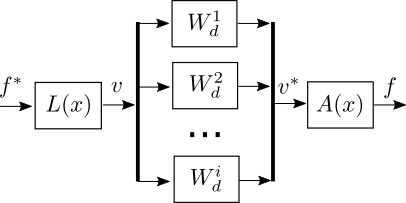
\includegraphics{./src/slau.png}
\end{figure}
}

, где $L$ - линейный решатель, а $x$ - вектор состояния системы в целом. 

Линейный решатель является вычислительной сущностью, реализуемой как часть контроллера $C(s,x)$, рассмотренного выше.

Переменные матричные коэффициенты $L$ и $A$ задают прямое и обратное координатное преобразование, Если рассматривать их в таком ключе, то группа органов управления напоминает по свойствам уже рассмотренные выше координатные домены, с той лишь разницей, что данное преобразование в общем случае меняет мерность системы. Как и в случае с вращающимися доменами, здесь проявляются нелинейные эффекты, которые тем ниже, чем меньше отношение постоянной времени органов управления к постоянным времени регуляторов САР и чем медленнее изменяется матрица $A(x)$. Если матрица $A$ является константой, нелинейные эффекты не проявляются. 

Данная система будет достигать наилучшего управления, если передаточные функции органов управления близки или каким-либо образом скомпенсированы. Исходя из этого соображения лучше объединять в группы органы управления схожей физической природы.

## Изменяемость векторов чувствительности в линейных группах органов управления.

Вектора чувствительности органов управления не являются константами в общем случае. В случае, когда объектом является манипулятор это имманентное свойство, поскольку геометрия манипулятора изменяется в процессе его работы, а следовательно изменяются операторы переноса. 

Для дронов же вектора чувствительности могут быть постоянными, но возможны также варианты с изменяемыми векторами тяги. В этом случае существует отдельная система управления, корректирующая направление вектора тяги.

В случае наличия изменяемых векторов тяги, система получает возможность корректировать матрицу чувствительности с тем, чтобы достигать наиболее оптимальной конфигурации при заданном желаемом управлении.

Вектор чувствительности можно считать оптимально направленным, когда его направление совпадает с направлением вектора желаемого управления. 

Для совмещения вектора чувствительности, в условиях, когда возможно управлять положением вектора тяги, следует задать движение направления вектора тяги по градиенту к вектору перенесённому обратным оператором переноса вектору желаемого управления. Такое управление может быть выполнено дополнительной следящей системой в рамках системного подхода, при этом в каждый момент времени управление тягой рассчитывается из текущей матрицы чувствительности независимо от динамики систем, решающих совмещения.

## Вырожденная линейная группа органов управления.



